\documentclass[a4paper, 12pt, titlepage]{article}
\usepackage{times}
\usepackage[utf8]{inputenc}
\usepackage[czech]{babel}
\usepackage[left=2cm, top=3cm, text={17cm, 24cm}]{geometry}
\usepackage[unicode]{hyperref}
\usepackage{graphicx}
\usepackage{float}
\urlstyle{same}


\begin{document}

\begin{titlepage}
\begin{center}
\textsc{\Huge
Vysoké učení technické v~Brně\\[0.3em]
\huge Fakulta informačních technologií}\\
\vspace{\stretch{0.382}}
{\LARGE Počítačové komunikace a sítě – 2. projekt\\[0.3em]
\Huge Síťový analyzátor}\\
\vspace{\stretch{0.618}}
\end{center}
{\Large \today \hfill Michal Sova}
\end{titlepage}

\tableofcontents
\newpage

\section{Implementace}
Analyzátor nejdříve zpracuje argumenty programu\cite{getopt}. Otevře rozhraní pro zachytávání paketů, nastaví filtr a pomocí funkce \verb|pcap_loop| a \verb|callback| funkce\cite{pcap}. V~\verb|callback| funkci nejdříve zkontroluje verzi IP, poté podle příslušné verze zavolá funkci \verb|getAddress|. Tato funkce zjistí z IP nebo IPv6 hlavičky typ protokolu zdrojovou a cílovou adresu a velikost IP hlavičky. Podle typu protokolu se získá z TCP nebo UDP zdrojový a cílový port. Následně vše vypíše na výstup. Výpis paketu je mezerou rozdělen na hlavičku a zbytek paketu.

\subsection{IP}
V IP hlavičce se analyzátor zaměřuje především na verzi(4 bity). Dále se zaměřuje na velikost hlavičky(4 bity), která po vynásobení 4 udává velikost IP hlavičky v bajtech.
Analyzátor také vyčte z hlavičky zdrojovou IP adresu, cílovou IP adresu a typ další hlavičky (TCP/UDP).
\renewcommand{\figurename}{Obrázek}
\begin{figure}[H]
    \centering
    \scalebox{0.39}{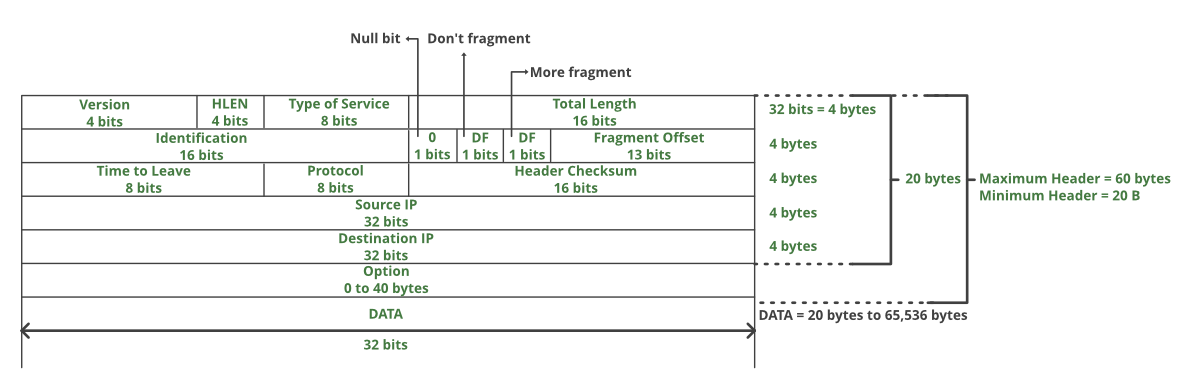
\includegraphics{ip-v4-datagram-header.png}}
    \caption{Hlavička IPv4\cite{obr1}}
    \label{obrazek 1}
\end{figure}
\subsection{IPv6}
IPv6 má pevnou velikost hlavičky, která je 40 bajtů. Analyzátor pro určení další hlavičky se dívá na Next Header, kde by tato informace měla být obsažená.
\begin{figure}[H]
    \centering
    \scalebox{0.45}{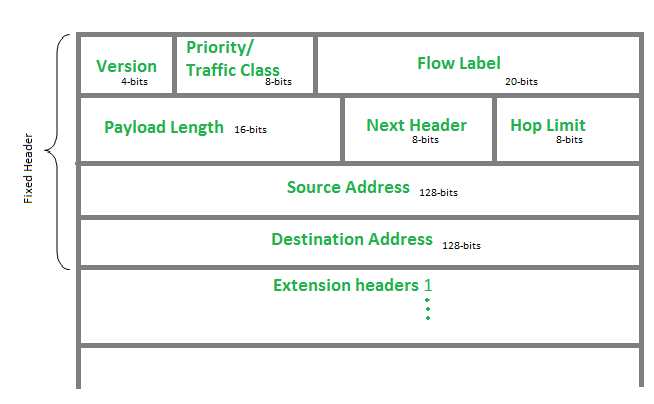
\includegraphics{ipv6-header.png}}
    \caption{Hlavička IPv6\cite{obr2}}
    \label{obrazek 2}
\end{figure}
\subsection{Transmission Control Protocol a User Datagram Protocol}
V hlavičkách TCP a UDP protokolů lze nalézt zdrojové a cílové porty. TCP a UDP protokoly by měly mít konstantní, avšak velikostně různé, hlavičky.

\section{využití knihoven}

Bylo využito knihovny pcap.h a jejich funkcí pro zachytávaní paketů. Knihovny netinet/ip.h\cite{ip} pro použití struktury \verb|struct ip|, ze které analyzátor načítá adresy a kontroluje další hlavičku. Podobně díky knihovně netinet/ip6.h\cite{ip6} a struktuře \verb|struct ip6_hdr|. Z~knihoven netinet/tcp.h\cite{tcp} a netinet/udp.h\cite{udp} byly využity struktury \verb|struct tcphdr| a \verb|struct udphdr|. 

\section{Testování}
K testování bylo využito nástroje Wireshark\footnote{\url{https://www.wireshark.org}}.
\subsection{Příklad testu}
Na Wiresharku byl nastaven filtr: \verb|(tcp port 8080) or (udp port 8080)| na rozhraní \verb|wlo1| a program byl spuštěn s následujícími parametry: \verb|./ipk-sniffer -i wlo1 -p 8080| pro vyfiltrování stejných paketů. Poslání paketu na tomto portu bylo vyvoláno příkazem curl, konkrétně: \verb|curl "http://seznam.cz:8080"|.

\begin{figure}[H]
    \centering
    \scalebox{0.25}{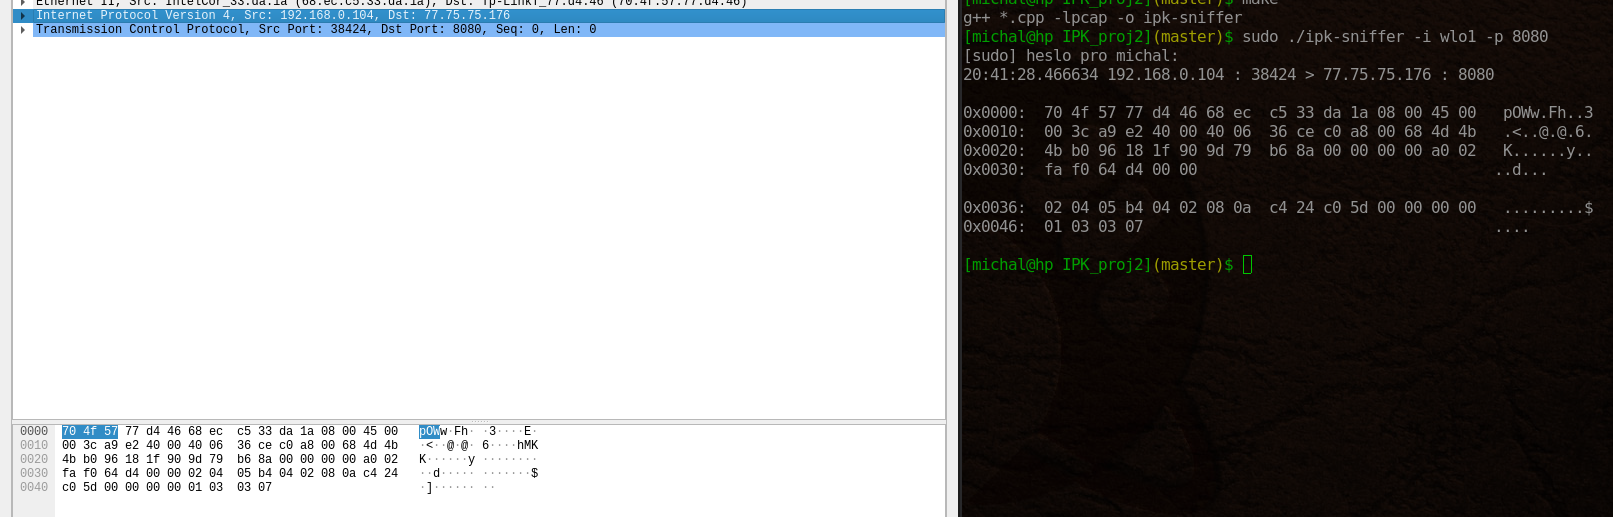
\includegraphics{ipk.png}}
    \caption{Příklad testu}
    \label{obrazek 3}
\end{figure}

Jak lze vidět na obrázku \ref{obrazek 3} pakety jsou stejné, pomineme-li odsazení hlavičky. Rovněž adresy a porty jsou stejné.

\newpage
\section{Použité zdroje}
\begin{thebibliography}{99}
\bibitem{getopt} Ashwin, V., 2015. How To Parse Program Options In C++ Using Getopt\_Long. [online] Code Yarns. Dostupné z:\url{https://codeyarns.com/2015/01/30/how-to-parse-program-options-in-c-using-getopt\_long/}
\bibitem{pcap} Carstens, T., 2020. Programming With Pcaptcpdump/LIBPCAP Public Repository. [online] Tcpdump.org. Dostupné z: \url{https://www.tcpdump.org/pcap.html}
\bibitem{ip} Unix.superglobalmegacorp.com. n.d. Netinet/Ip.H Source. [online] Dostupné z: \url{https://unix.superglobalmegacorp.com/Net2/newsrc/netinet/ip.h.html}
\bibitem{ip6} Code.woboq.org. n.d. Ip6.H Source Code [Glibc/Inet/Netinet/Ip6.H] - Woboq Code Browser. [online] Dostupné z: \url{https://code.woboq.org/userspace/glibc/inet/netinet/ip6.h.html}
\bibitem{tcp} Unix.superglobalmegacorp.com. n.d. Netinet/Tcp.H Source. [online] Dostupné z: \url{https://unix.superglobalmegacorp.com/BSD4.4/newsrc/netinet/tcp.h.html}
\bibitem{udp} Unix.superglobalmegacorp.com. n.d. Netinet/Udp.H Source. [online] Available at: \url{https://unix.superglobalmegacorp.com/Net2/newsrc/netinet/udp.h.html}
\end{thebibliography}

\subsection{Obrázky}
\begin{thebibliography}{99}
\bibitem{obr1} GeeksforGeeks. n.d. Introduction And Ipv4 Datagram Header - Geeksforgeeks. [online] Dostupné z: \url{https://www.geeksforgeeks.org/introduction-and-ipv4-datagram-header/}
\bibitem{obr2} GeeksforGeeks. n.d. Internet Protocol Version 6 (Ipv6) Header - Geeksforgeeks. [online] Dostupné z: \url{https://www.geeksforgeeks.org/internet-protocol-version-6-ipv6-header/}
\end{thebibliography}

\newpage

\section{Upřesnění chování analyzátoru}
\begin{itemize}
    \item Analyzátor ignoruje neznámé argumenty.
    \item Analyzátor podporuje je protokoly tcp a udp.
    \end{itemize}
\subsection{Omezení}
\begin{itemize}
  \item Analyzátor nepřekládá IP adresy na doménové jména.
\end{itemize}

\end{document}
